\chapter{Evaluation}
\chaplabel{evaluation}

In diesem Kapitel geht es um die Bewertung der Vorverarbeitung und die durchgeführten Experimente. Die zur Evaluation der Vorverarbeitung, des genutzten ML-Algorithmus und der Experimente benötigten Metriken werden erläutert. Die jeweiligen Ziele und Ergebnisse dieser Experimente werden in diesem Kapitel vorgestellt.

Die einzelnen Experimente lassen sich in 3 Phasen einteilen, die sich sowohl in der Anzahl der genutzten Finger als auch der zu lernenden Tasten unterscheiden. Das Ziel der verschiedenen Versuche ist es, die Einstellungen des Netzes anzupassen und zu verbessern, aber auch die Einschränkungen und Grenzen des Datenhandschuhs und der verwendeten ML-Methoden zu ermitteln.

\section{Vorverarbeitung}

\begin{figure}[p]
    \centering
    \advance\leftskip-2cm
    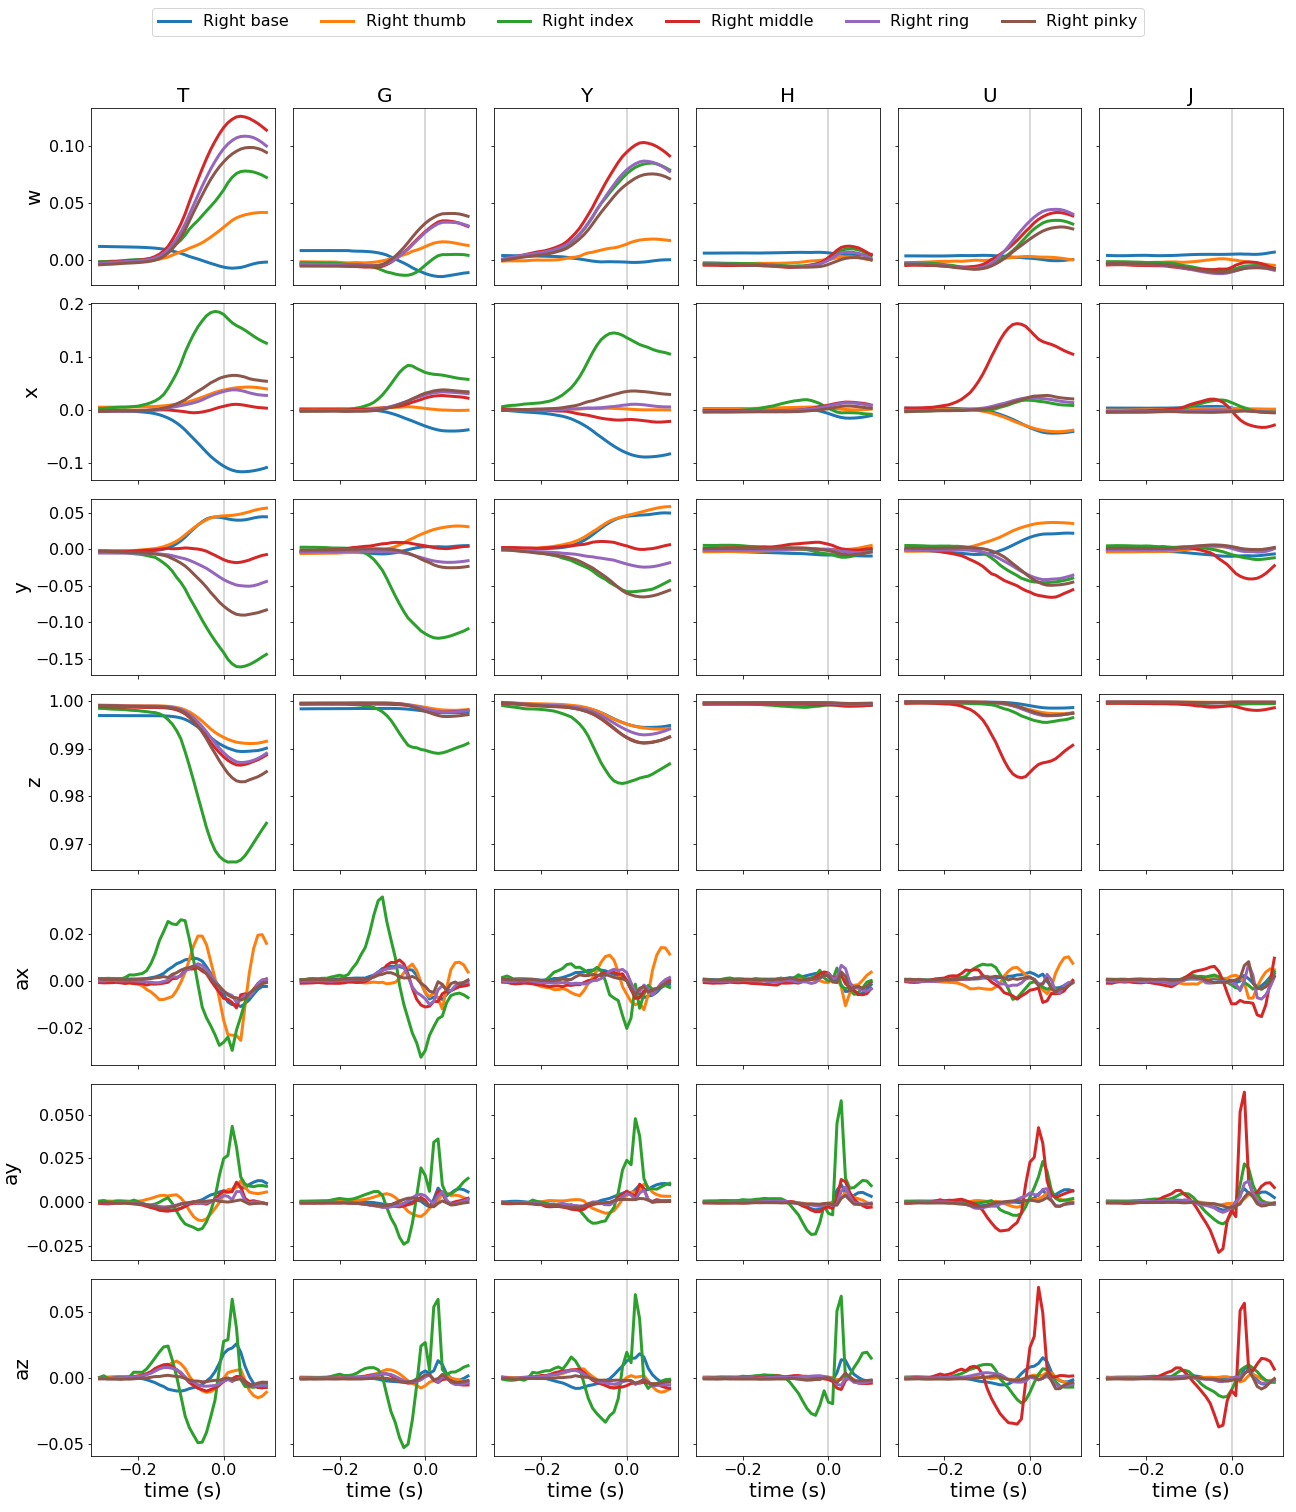
\includegraphics[width=17cm]{../common/images/graphs-average}
    \caption[Durchschnittswerte verschiedener Tasten]{Durchschnittswerte der Orientierungs- und Beschleunigungsdaten über je ca. 150 Tastendrücke der in Phase 2 aufgezeichneten Tasten. Die X-Achse zeigt die vergangene Zeit vor und nach dem Tastenanschlag, die Y-Achse zeigt die jeweiligen Werte der Quaternion und des Accelerometers.}
    \label{fig:graphs-average}
\end{figure}

Die Vorverarbeitung der Daten erwies sich als sehr sinnvoll und gut geeignet, um den Lernprozess zu vereinfachen. In \figref{graphs-average} sind die von uns erhofften Muster für verschiedene Tastendrücke in den vorverarbeiteten Bewegungsdaten deutlich zu erkennen.

In den einzelnen Graphen sind die durchschnittlichen Werte sowohl der Quaternionen als auch der Accelerometerdaten einiger Tasten\footnote{In Phase 2 werden insgesamt 10 Tasten für das Lernen verwendet. Die Abbildung zeigt jedoch lediglich sechs dieser Tasten, um die Übersichtlichkeit zu gewährleisten.} aus Phase 2 zu sehen. Die X-Achse beschreibt die vergangene Zeit vor und nach einem Tastendruck. Dieser ist mit einer vertikalen grauen Linie gekennzeichnet. Auf der Y-Achse stehen die gesamten Werte der Quarternions (von oben nach unten: w, x, y, z) und des Accelerometers (ax, ay, az) nach Durchlaufen der Vorverarbeitung. Zusätzlich zum Vorverarbeiten wurden die durchschnittlichen Werte aller aufgenommenen Tastendrücke der jeweiligen Taste errechnet und im Graphen als jeweils eine Linie abgebildet.

Aus den Graphen wird ersichtlich, dass die verschiedenen Tasten gut zu unterscheiden sind. Bei einigen Tasten sind diese Unterschiede deutlich zu erkennen, wie zum Beispiel bei den Tasten \keyboard{T} und \keyboard{J}. Diese Tasten sind auf der Tastatur relativ weit voneinander entfernt und benötigen für das Tippen eindeutig unterscheidbare Fingerbewegungen. Doch auch bei den auf den ersten Blick sehr ähnlich aussehenden Mustern einiger Tasten, können bei genauer Betrachtung Unterschiede festgestellt werden.

Als Beispiel sollen hier die Tasten \keyboard{H} und \keyboard{J} dienen. Da sich beide Tasten in der mittleren Tastenreihe befinden, sind die Fingerbewegungen zum Drücken der Tasten sehr gering. Dennoch werden diese Bewegungen mit unerschiedlichen Finger getätigt. Die Unterschiede in den Quaterniondaten sind eher gering. Auf der y- und auch der z-Achse der Accelerationsdaten schlagen jedoch bei \keyboard{H} die Werte des Zeigefinger und bei \keyboard{J} die Werte des Mittelfingers deutlich aus. Da dies der Fall ist, scheint die zusätliche Nutzung der Accelerometerdaten sinnvoll zu sein.

\section{Metriken zur Evaluation des Modells}\seclabel{metriken}

Geeignete Metriken zu finden, um das gelernte Netz bewerten zu können, ist für überwachtes Lernen unabdingbar und sowohl für den Lernprozess, als auch die spätere Analyse sehr wichtig.

Zunächst werde ich auf die Kostenfunktion eingehen. Diese wird beim Lernen verwendet, um zu ermitteln wie gut die gemachten Prädiktionen sind. Hierfür werden die vom Netz ermittelten Werte mit den tatsächlichen Zielwerten verglichen, um dann die Kanten des neuronalen Netzes entsprechend der gemachten Fehler (Kosten) anzupassen.

Wie in \secref{konfig} ,,Konfiguration'' erwähnt, haben wir für das CNN den Mean Squared Error als Kostenfunktion verwendet. Dieser errechnet sich aus den Vorhersagen $pred$ und den Zielwerten $act$:

$$\text{MSE}(pred, act) := \frac{1}{n} \cdot \sum_{i=0}^{n} (pred_i - act_i)^2$$

Es wird hierbei für jedes Sample die Differenz zwischen den jeweils $n$ ermittelten und tatsächlichen Zielwerten quadriert. Diese Differenzen werden aufsummiert und durch die Anzahl der Werte geteilt.

Die erhaltenden Werte werden als Kosten angesehen. Im Backpropagation-Schritt werden die Kanten angepasst, um die Kosten zu reduzieren. Diese Anpassung fällt je nach eingestellter Lernrate mehr oder weniger groß aus und ist abhängig von der jeweiligen Kante.

Zur Evaluation eines Klassifizerungs-Algorithmus wird oft die sogenannte Confusion Matrix (siehe \tabref{confusion}) zur Hilfe genommen. In dieser Matrix wird festgehalten, wie oft die verschiedenen Klassen vorkamen und als welche Klasse sie erkannt wurden. Links stehen die tatsächlichen, oben die vom Klassifikator ermittelten Klassen.

Meist wird die Confusion Matrix für lediglich zwei Klassen verwendet. Hierbei kann in 4 Kategorien eingeteilt werden, jeweils zwei für richtige und zwei für falsche Klassifikationen.

\begin{table}[htb]
    \centering
    \subcaptionbox[0.8\textwidth]{Confusion Matrix; (TP) korrekt als positiv, (FN) falsch als negativ, (FP) falsch als positiv und (TN) korrekt als negativ erkannte Klassen.\tablabel{confusion}}{
        \centering
        \begin{tabular}{c|c|c|c|}
    \multicolumn{2}{c}{} & \multicolumn{2}{c}{\textbf{Predicted}} \\ \cline{3-4}
    \multicolumn{2}{c|}{}
        & \makecell{Class 1 \\[-4pt] \scriptsize positive}
        & \makecell{Class 2 \\[-4pt] \scriptsize negative}
        \\ \cline{2-4}
    \multirow{2}{*}{\rotatebox[origin=c]{90}{\textbf{Actual}}}
        & \makecell{Class 1 \\[-4pt] \scriptsize positive}
        & \makecell{TP}
        & \makecell{FN}
        \\ \cline{2-4}
    % nothing here
        & \makecell{Class 2 \\[-4pt] \scriptsize negative}
        & \makecell{FP}
        & \makecell{TN}
        \\ \cline{2-4}
\end{tabular}

    }

    \vspace{2em}

    \subcaptionbox[0.8\textwidth]{Übliche Metriken, welche aus einer Confusion Matrix ablesbar sind; $n$ ist hier die Größe der Testmenge\tablabel{metriken}}{
        \centering
        {
\renewcommand*{\arraystretch}{1.6}
\begin{tabular}{@{}llp{8cm}@{}}
    \toprule
    \textbf{Metrik} & \textbf{Formel} & \textbf{Fragestellung} \\
    \midrule
    Accuracy
        & $\frac{\text{TP} + \text{TN}}{n}$
        & Anteil korrekter Vorhersagen \\
    Recall
        & $\frac{\text{TP}}{TP + FN}$
        & Anteil korrekter Vorhersagen in der positiven Klasse \\
    Precision
        & $\frac{\text{TP}}{TP + FP}$
        & Anteil der als positiv vorhergesehenen Samples, der korrekt war \\
    F-Score
        & $\frac{2 \text{ PR}}{P + R}$
        & harmonisches Mittel aus Recall (R) und Precision (P), \citet{f-measure} \\
    \bottomrule
\end{tabular}
}

    }

    \caption{Confusion Matrix mit zwei Klassen und daraus ablesbare Metriken}
    \tablabel{confusion-metriken}
\end{table}

Wir verwenden die aus der Confusion-Matrix ableitbaren Werte der Accuracy, der Precision und des Recalls, sowie den F-Score (auch F1-Score genannt), um den Lernfortschritt und -erfolg des Experiments zu überwachen. In \tabref{metriken} sind diese Begriffe mit ihrer Formel und einer kurzen Beschreibung aufgelistet.

Bei der Accuracy handelt es sich um die Genauigkeit der Prädiktionen. Hierbei wird der Anteil der korrekt klassifizierten Samples berechnet. Die alleinige Verwendung der Accuracy ist in den meisten Fällen nicht zu empfehlen, da sie oft ein falschen Eindruck des Lernerfolgs vermittelt. Wie bereits erwähnt ist die Accuracy bei unbalancierten Datensätzen oft sehr schnell am optimalen Wert, beispielsweise wenn der Klassifikator jedes Sample der negativen Klasse zuordnet. Da diese Klasse einen sehr großen Teil der Daten ausmacht, sind fast alle Samples korrekt klassifiziert, das Lernen war jedoch trotzdem kein Erfolg.

Der Recall beschreibt den Anteil der korrekt erkannten Samples der positiven Klasse. Dieser Wert ist in Verbindung mit der Precision besonders aussagekräftig, da diese sicher\-stellt, dass nicht übermäßig oft Samples der positive Klasse zugeordnet werden. Sie berechnet den Anteil der als positiv klassifizierten Samples, welche auch tatsächlich zur positiven Klasse gehören.

Der F-Score verbindet Recall und Precision zu einem Wert und ist dadurch gut geeignet, um Rückschlüsse auf den Lernerfolg ziehen zu können, auch wenn mit unbalancierten Daten gelernt wurde.

In mehrklassigen Problemen lassen sich Recall, Precision und F-Score nur in Bezug auf jeweils eine Klasse angeben. Daher errechnen wir für jede unserer zu erkennenden Tasten getrennt diese Metriken. Wir überwachen diese über den Lernprozess und zeichnen daraus Graphen, um zu erkennen, ob sich der Klassifikator dem Optimum von jeweils 100\% annähert.

\section{Phase 1: Erkennen einer Taste}

In der ersten Phase erstellten wir einen Datensatz, in dem die Testperson mit dem Zeigefinger der rechten Hand, an welcher der Datenhandschuh befestigt war, in zufälliger Reihenfolge die zwei Tasten \keyboard{N} und \keyboard{K} drückte (\figref{keyboard-phase-1}). Hierbei ist die eher ungewöhnliche Ruheposition der Hand der Testperson zu erwähnen. Der Zeigefinger der Testperson liegt auf der Taste \keyboard{H} und nicht, wie üblich, auf der Taste \keyboard{J}. Zudem wurde ein US-Tastaturlayout verwendet.

Die Fingerbewegungen wurden sehr langsam ausgeführt, mit kleinen Pausen zwischen den einzelnen Bewegungen. Nach jeder Bewegung wurden die Finger wieder in die Ausgangsposition bewegt.

\begin{figure}[h]
    \centering
    \phasekeyboard{1}
    \caption[Tasten und Finger in Phase 1]{Verwendete Tasten und Finger in Phase 1.}
    \figlabel{keyboard-phase-1}
\end{figure}

In dieser Phase wollten wir ermitteln, ob die einzelnen Tastenanschläge in den Daten überhaupt erkennbar sind und ob ein neuronales Netz in der Lage ist, das Rauschen in den Daten zu ignorieren und die Fingerbewegungen für das Drücken einer Taste zu registrieren. Wir wollten herauszufinden, ob selbst direkt benachbarte Tasten unterscheidbar sind.

\begin{figure}
    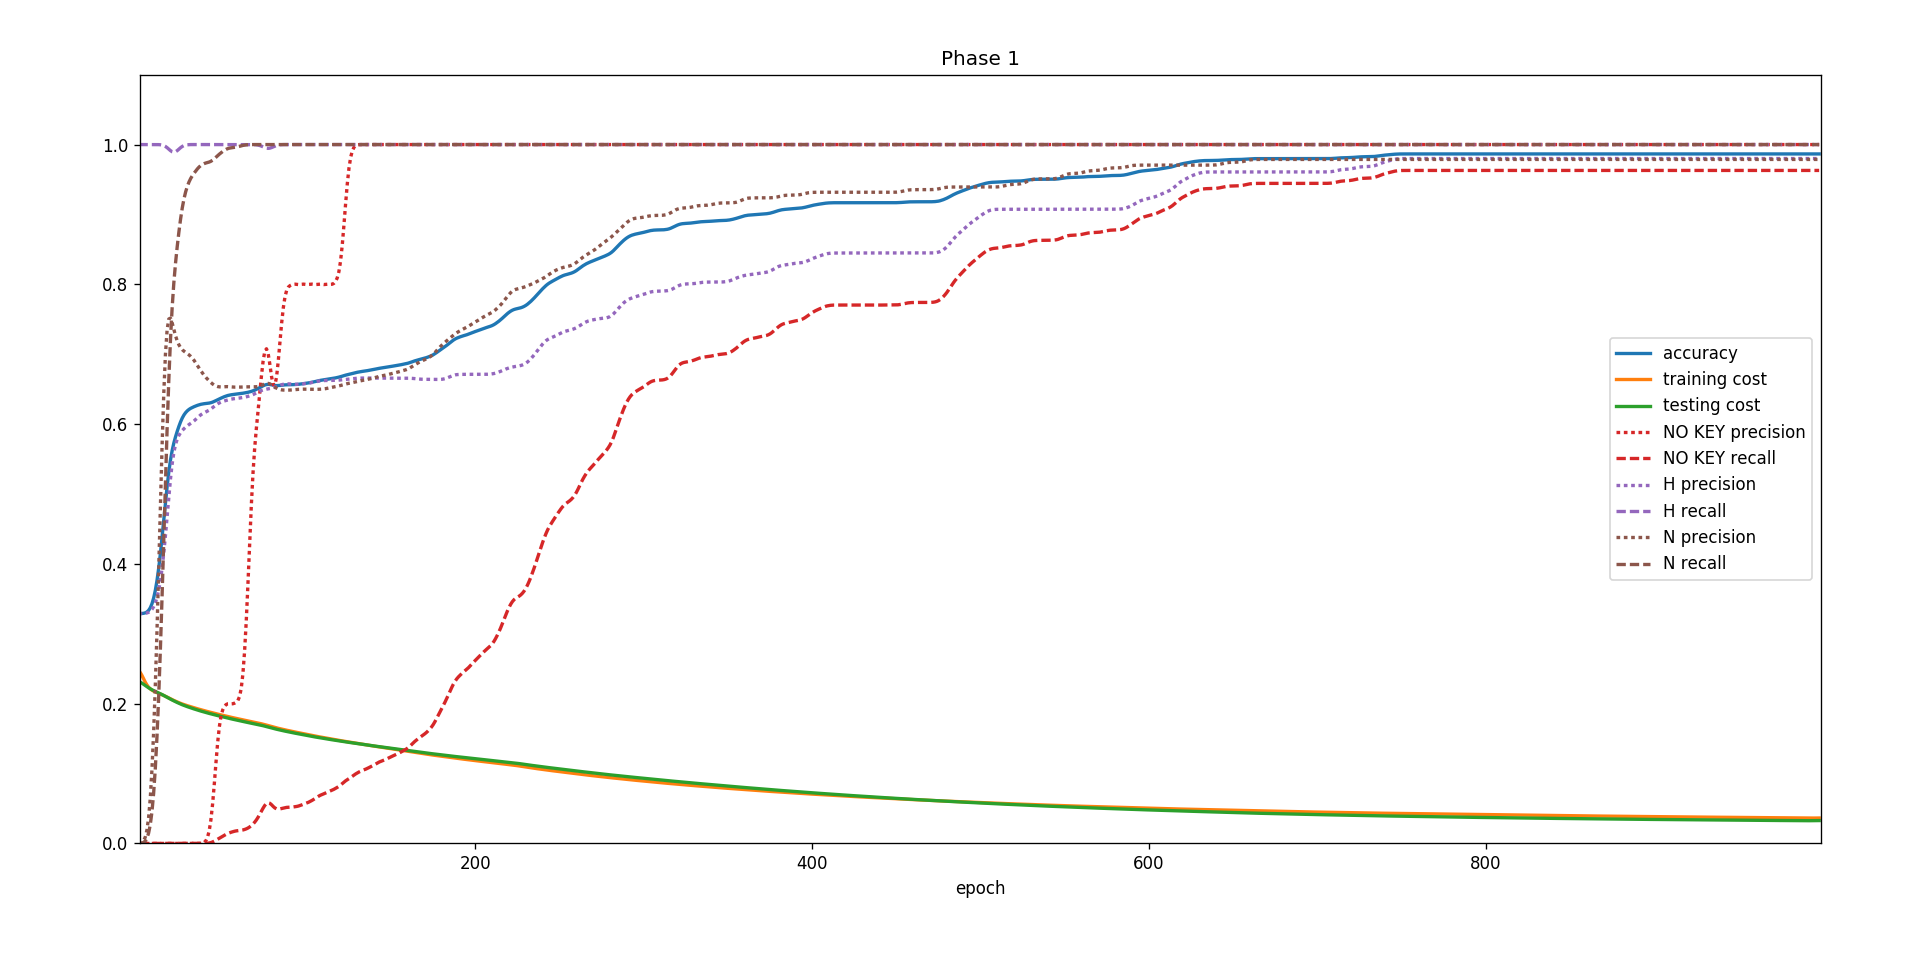
\includegraphics[width=\textwidth]{../common/images/phase-1-detailed.png}
    \caption[Testergebnisse Phase 1]{Testergebnisse der Phase 1 in den ersten \num{1000} Epochen. Die Accuracy liegt bei knapp 97\%, die Klasse $\emptyset$ wird langsamer gelernt als die anderen.}
    \figlabel{phase1}
\end{figure}

In \figref{phase1} ist die Entwicklungskurve der Accuracy und der Trainings- und Testkosten beim Lernen des Netzes mit dem oben beschriebenem Datensatz zu sehen. Nach \num{1000} Epochen ist bereits eine Accuracy von ungefähr 97\% erreicht, die Kosten wurden sowohl beim Trainings- als auch beim Testdatensatz stark reduziert.

Außerdem sind Precision und Recall aller Klassen eingezeichnet. Hierbei ist zu erkennen, dass der Recall der Klasse $\emptyset$ relativ spät optimiert wird, stattdessen werden die dieser Klasse zugehörigen Samples zuvor den anderen Klassen zugeordnet.

Wir waren mit dem so trainierten Modell in der Lage, Tippbewegungen auf einem Tisch durchzuführen, welche dem Tippen auf diesen Tasten ähnelten. Das neuronale Netz konnte diese Tippbewegungen zuverlässig erkennen. Je nach Beugungsgrad des Zeigefingers wurde \keyboard{N} oder \keyboard{H} erkannt.

\section{Phase 2: Differenzieren verschiedener Tasten}

Für die zweite Phase wurden drei Finger und ingesamt 10 verschiedene Tasten verwendet.

\begin{figure}[h]
    \centering
    \phasekeyboard{2}
    \caption[Tasten und Finger in Phase 2]{Verwendete Tasten und Finger in Phase 2. Mit dem Daumen, dem Zeige- sowie dem Ringfinger werden insgesamt 10 verschiedene Tasten gedrückt.}
    \figlabel{keyboard-phase-2}
\end{figure}

In dieser Phase legen wir unter anderem Wert darauf, die Vorverarbeitung der Daten zu verbessern und dadurch das Lernen zu erleichtern.

Um zum Beispiel die Taste \keyboard{T} zu drücken, muss im Gegensatz zur vorherigen Phase die Handposition verändert werden. Die Daten der Hand-IMU sollten helfen, diese Handbewegungen zu erkennen und genauere Rückschlüsse auf die getippte Taste ziehen zu können.

Ein besonderes Augenmerk liegt auf den Tasten der \fremdwort{mittleren Tastenreihe}. Als mittlere Tastenreihe bezeichne ich die Tasten, welche von den Fingern bedeckt werden, wenn die Hand in der Ruheposition auf der Tastatur liegt. Zum Tippen dieser Tasten ist lediglich eine minimale Bewegung der Finger erforderlich. Dies macht die Erkennung dieser Tasten anhand der Bewegungsdaten schwieriger als die der anderen Tasten.

Die Testperson hat den Zeigefinger in der Ruheposition auf der Taste \keyboard{H} liegen. Dadurch sind die Tasten \keyboard{H}, \keyboard{J}, \keyboard{K}, \keyboard{L} und \keyboard{\spacebar} in der mittleren Tastenreihe enthalten.

Wie in \figref{keyboard-phase-2} zu sehen, sind in dieser Phase drei Tasten der mittleren Tastenreihe zu lernen. Dadurch können wir bestehende Schwierigkeiten durch den geringen Bewegungsaufwand erkennen und Lösungswege evaluieren.

In dieser Phase haben wir mehrere Experimente durchgeführt.
Im ersten Experiment erzielten wir eine Genauigkeit von knapp 76\%, was eine deutliche Verschlechterung im Vergleich zu der ersten Phase darstellte, obwohl mit \num{160000} Epochen deutlich mehr Epochen gelernt wurden.
Die Confusion Matrix in \figref{confusion_matrix} half uns die für die schlechte Accuracy ausschlaggebenden Tasten zu identifizieren.

\begin{figure}
    \centering
    \pgfkeys{/pgf/declare function={rescale(\x) = (\x*2-1)^3*0.5+0.5;}}

\begin{tikzpicture}[
    square/.style={
        inner sep=0pt,
        rectangle,
        minimum width=1cm,
        minimum height=0.5cm,
        anchor=north west,
    },
    every node/.style={
        font=\scriptsize,
    },
]
    % \node[inner sep=2pt,circle,fill=green] at (0, 0) {};
    \node[inner sep=0pt,rectangle,anchor=south east,rotate=90,minimum width=5cm,minimum height=0.5cm,draw,xshift=0.5\pgflinewidth,thick]
        at (0, -0.5) {\bfseries{}Actual};
    \node[inner sep=0pt,rectangle,anchor=south west,minimum width=10cm,minimum height=0.5cm,draw,xshift=-0.5\pgflinewidth,thick]
        at (1, 0) {\bfseries{}Predicted};

    \foreach \row [count=\y] in {{0,13,5,9,5,121,2,6,3,0},{0,175,0,0,0,0,0,0,0,0},{0,1,167,0,0,0,0,0,0,0},{0,0,0,181,0,0,0,0,0,0},{0,1,5,0,1,169,0,0,0,0},{0,0,1,0,1,215,0,3,0,0},{0,0,0,0,0,0,167,0,0,0},{0,0,0,0,0,0,0,180,0,0},{0,0,0,0,0,0,0,0,190,0},{0,0,0,0,4,178,1,0,0,0}} {
        \foreach \v [count=\x] in \row {
            \pgfmathsetmacro{\tmp}{\v/215.0}
            \pgfmathtruncatemacro{\back}{rescale(\tmp)*100}
            \pgfmathtruncatemacro{\fore}{(\tmp>0.5)*100}
            \node[square,fill=black!\back!white,text=white!\fore!black] at (\x,-\y*0.5) {$\v$};
        }
    }

    \foreach \key [count=\i] in {$\emptyset$,Y,U,G,H,J,B,N,M,\textvisiblespace} {
        \node[square] at (0, -(\i*0.5) {\bfseries\key};
        \node[square] at (\i, 0) {\bfseries\key};
    }

    \foreach \i in {2,...,10} {
        \draw[draw,dotted] (\i, 0) -- (\i, -5.5);
        \draw[draw,dotted] (0, -\i*0.5) -- (11, -\i*0.5);
    }

    \foreach \i in {1,11} {
        \draw[draw,thick] (\i, 0) -- (\i, -5.5);
        \draw[draw,thick] (0, -\i*0.5) -- (11, -\i*0.5);
    }
\end{tikzpicture}

    \caption[Confusion Matrix des ersten Experiments der Phase 2]{Confusion Matrix des ersten Experiments der Phase 2. \keyboard{H}, \keyboard{\spacebar} und $\emptyset$ werden nicht gut erkannt, in den meisten Fällen wird stattdessen \keyboard{J} erkannt\footnotemark.}
    \figlabel{confusion_matrix}
\end{figure}

Die Tasten \keyboard{Y}, \keyboard{U}, \keyboard{G}, \keyboard{B}, \keyboard{N} und \keyboard{M} wurden mit nur wenigen falschen Prädiktionen sehr gut erkannt.
Die Tasten \keyboard{H}, \keyboard{\spacebar} und auch das Fehlen eines Tastendrucks, also $\emptyset$, wurden fast nie richtig erkannt. Stattdessen wurde die meisten Samples aus diesen Klassen dem Druck der Taste \keyboard{J} zugeordnet.
Wir kamen zu dem Schluss, dass die Tastatur und die dadurch resultierenden Fingerbewegungen Grund hierfür sein können.
% Die Tasten, auf denen die Finger in der Ruhepositionen liegen, werden im Folgenden mittlere Tastenreihe genannt.

Bei den erwähnten Tasten handelt es sich ausschließlich um die Tasten, die sich in der mittleren Tastenreihe befinden. Um diese zu drücken, müssen sich die Finger also nicht von der Ruheposition wegbewegen, sondern lediglich die unter dem Finger befindliche Taste hinunterdrücken. Ähnliche Beobachtungen konnten, wie bereits erwähnt, in der Confusion Matrix von \citet{nasa-joystick-keyboard} gemacht werden.

Da zum Aufzeichnen eine sehr flache Tastatur verwendet wurde, die bereits mit sehr geringem Druck auslöst, war die Fingerbewegung für das Tippen einer dieser Tasten sehr gering und das CNN nicht in der Lage diese zu differenzieren.

\footnotetext{Diese Matrix enthält aufgrund eines Konfigurationsfehlers im ersten Experiment nicht alle Tasten wie geplant. Dies haben wir im nachfolgenden Experiment korrigiert.}

\begin{figure}
    \centering
    \pgfkeys{/pgf/declare function={rescale(\x) = (\x*2-1)^3*0.5+0.5;}}

\begin{tikzpicture}[
    square/.style={
        inner sep=0pt,
        rectangle,
        minimum width=1cm,
        minimum height=0.5cm,
        anchor=north west,
    },
    every node/.style={
        font=\scriptsize,
    },
]
    % \node[inner sep=2pt,circle,fill=green] at (0, 0) {};
    \node[inner sep=0pt,rectangle,anchor=south east,rotate=90,minimum width=5.5cm,minimum height=0.5cm,draw,xshift=0.5\pgflinewidth,thick]
        at (0, -0.5) {\bfseries{}Actual};
    \node[inner sep=0pt,rectangle,anchor=south west,minimum width=11cm,minimum height=0.5cm,draw,xshift=-0.5\pgflinewidth,thick]
        at (1, 0) {\bfseries{}Predicted};

    \foreach \row [count=\y] in {{39,3,5,4,4,31,6,6,55,5,22},{0,166,0,0,0,0,0,0,0,0,0},{0,1,180,0,0,0,0,0,0,0,0},{0,0,0,167,0,0,0,0,0,0,0},{0,1,0,0,174,0,0,0,0,0,0},{2,0,0,0,1,147,0,4,22,0,0},{2,0,0,0,0,0,177,1,0,0,0},{0,0,0,0,1,0,0,167,0,0,0},{8,0,0,0,0,26,3,0,179,0,4},{0,0,0,0,0,0,0,0,0,190,0},{4,0,0,0,0,0,0,0,0,0,179}} {
        \foreach \v [count=\x] in \row {
            \pgfmathsetmacro{\tmp}{\v/215.0}
            \pgfmathtruncatemacro{\back}{rescale(\tmp)*100}
            \pgfmathtruncatemacro{\fore}{(\tmp>0.5)*100}
            \node[square,fill=black!\back!white,text=white!\fore!black] at (\x,-\y*0.5) {$\v$};
        }
    }

    \foreach \key [count=\i] in {$\emptyset$,T,G,B,Y,H,N,U,J,M,\textvisiblespace} {
        \node[square] at (0, -(\i*0.5) {\bfseries\key};
        \node[square] at (\i, 0) {\bfseries\key};
    }

    \foreach \i in {2,...,11} {
        \draw[draw,dotted] (\i, 0) -- (\i, -6);
        \draw[draw,dotted] (0, -\i*0.5) -- (12, -\i*0.5);
    }

    \foreach \i in {1,12} {
        \draw[draw,thick] (\i, 0) -- (\i, -6);
        \draw[draw,thick] (0, -\i*0.5) -- (12, -\i*0.5);
    }
\end{tikzpicture} 
    \caption[Confusion Matrix des zweiten Experiments der Phase 2]{Confusion Matrix des zweiten Experiments der Phase 2. \keyboard{H}, \keyboard{J}, \keyboard{\spacebar} und $\emptyset$ werden wesentlich besser als zuvor erkannt, jedoch immer noch deutlich schlechter als die anderen Klassen.}
    \figlabel{confusion_matrix2}
\end{figure}

\begin{figure}
    \centering
    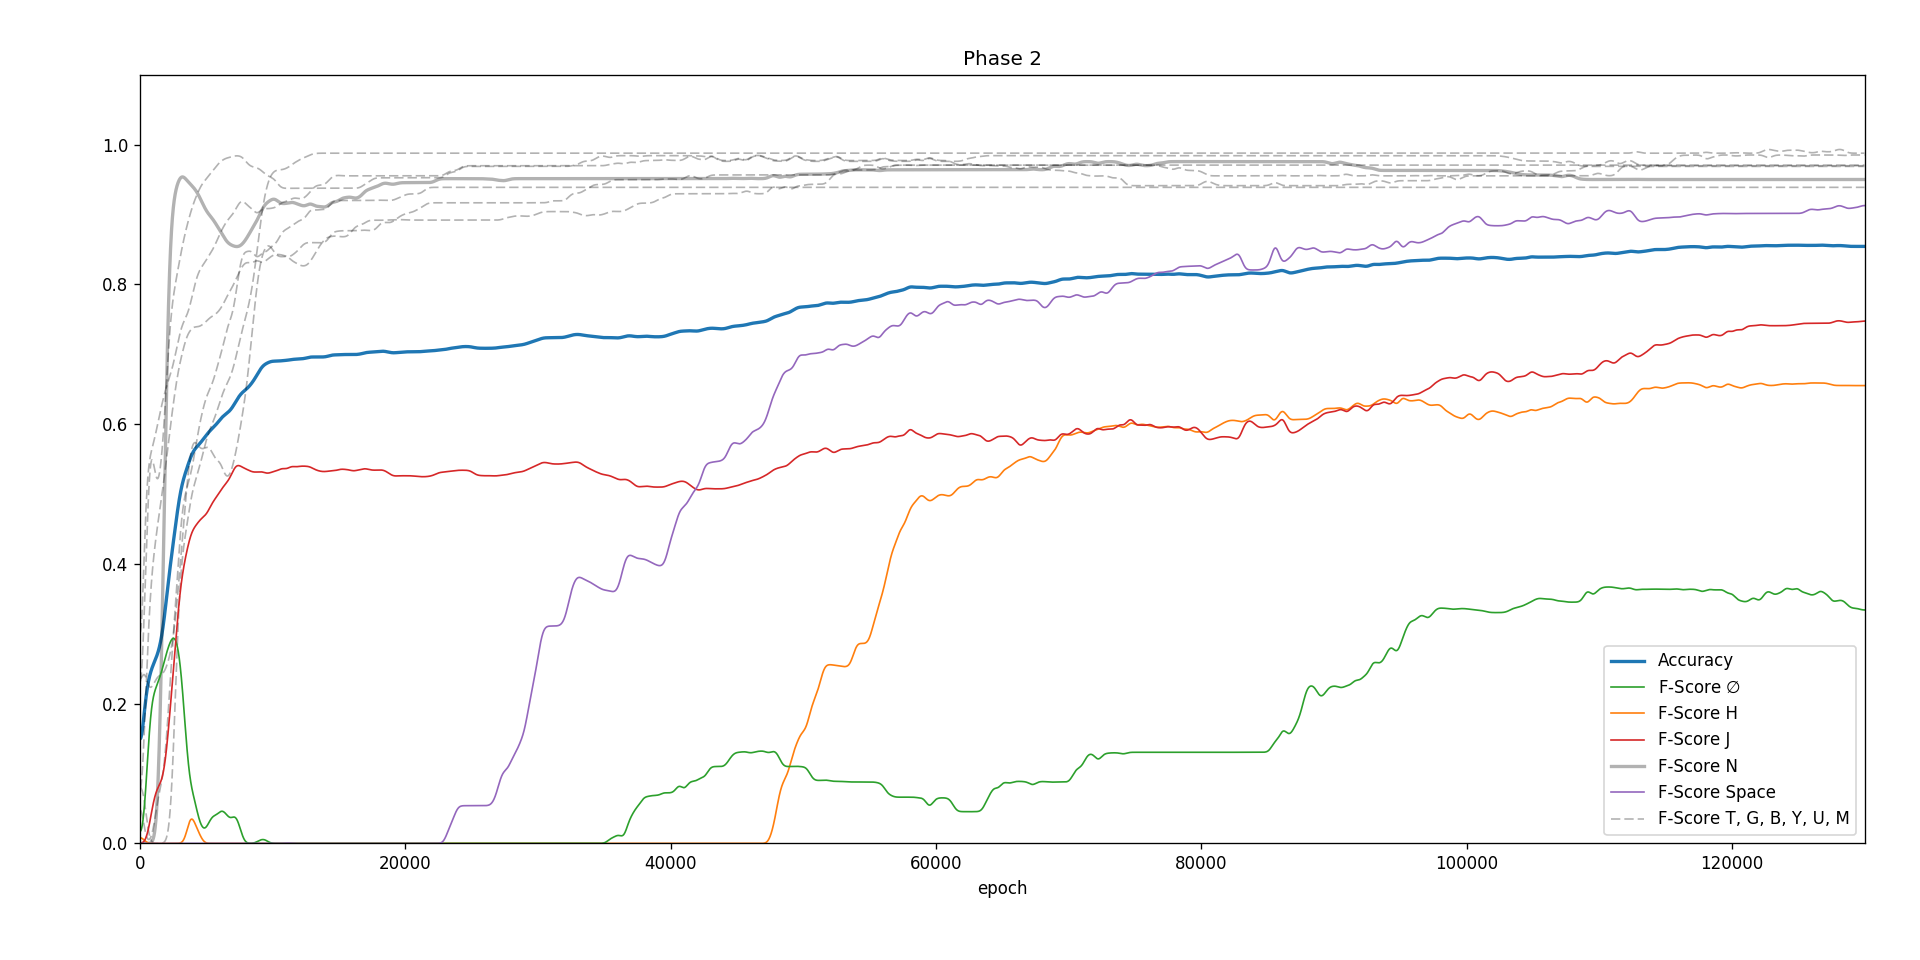
\includegraphics[width=\textwidth]{../common/images/phase2.png}
    \caption[Performance-Metriken des zweiten Experiments der Phase 2]{Performance-Metriken des zweiten Experiments der Phase 2 (\num{130000} Epochen). Die F-Scores der verwendeten Tasten sind in zwei Gruppen eingeteilt, Tasten der mittleren Tastenreihe sind farbig, die restlichen Tasten sind grau dargestellt. Hervorgehoben ist der F-Score der Taste N.}
    \figlabel{phase2_graph}
\end{figure}

Eine Wiederholung des Experiments erzielte jedoch ein besseres Ergebnis als der erste Durchlauf. Der erste Lernvorgang wurde demnach zu früh abgebrochen, obwohl er deutlich mehr Epochen benötigte, als der zweite. Dies liegt vermutlich daran, dass das Netz zu Beginn zufällig initialisiert wird und dadurch mit unterschiedlichen Voraussetzungen startet.

Die Confusion Matrix des zweiten Durchlaufs ist in \figref{confusion_matrix2} abgebildet. Die gewünschte Diagonale durch die Tabellenwerte ist hier deutlicher zu erkennen, als in der Confusion Matrix des ersten Experiments und ein Großteil der Samples der nicht auf der mittleren Tastenreihe befindlichen Tasten, werden mit wenigen Ausnahmen korrekt erkannt. Die Samples der Klasse $\emptyset$ werden allen anderen Klassen zugeordnet. Bei den Samples anderer Klassen sind höchstens fünf verschiedene Klassen in den Prädiktionen enthalten.
Das Erkennen der $\emptyset$-Klasse erfordert also eine gesonderte Optimierung.

In \figref{phase2_graph} ist der Ergebnisgraph des zweiten Experiments abgebildet.
Die grauen Linien stehen für die Tasten, welche sich schon im ersten Experiment als leicht erlernbar erwiesen. Die farbigen Linien gehören zu den Tasten der mittleren Tastenreihe. Ein direkter Vergleich der beiden Tastengruppen zeigt, dass die Tasten der mittleren Tastenreihe erst deutlich später gelernt werden als die anderen.

Am Beispiel der Tasten \keyboard{H} und \keyboard{N} wird das deutlich. Die Taste \keyboard{N} wird von Beginn an erkannt und erzielt schon bei ungefäher \num{20000} Epochen den F-Score von 95\%. Die Taste \keyboard{H} wird bis ungefähr zur \num{50000} Epoche ignoriert. Erst dann wird sie langsam erkannt und erreicht schließlich einen F-Score von 65.9\%, immer noch wesentlich schlechter als der von der Taste \keyboard{N}.
Insgesamt konnte eine Accuracy von 85\% erreicht werden, eine deutliche Verbesserung zum vorherigen Experiment mit 76\% Genauigkeit.

Da trotz des besseren zweiten Experiments die Tasten der mittleren Reihe deutlich schlechter abschneiden als die anderen, ist es sinnvoll, ein weiteres Experiment durchzuführen, bei der eine Tastatur verwendet wird, die ein deutlicheres Drücken erfordert.

Eine weiteres Experiment könnte die Daten des Accelerometers zum Lernen hinzunehmen. In \figref{graphs-average} ist zu sehen, dass diese Daten eine bessere Unterscheidung zwischen den Tasten der mittleren Tastenreihe ermöglichen.

Es sind auch noch weitere Verbesserungsmöglichkeiten aufgefallen, wie zum Beispiel die Verzögerung bei der Anwendung des gelernten Netzes.
Diese resultiert vor allem aus der Art der Sampling-Methode. Da wir die Tastendrücke in die Mitte der für ein Sample verwendeten Zeitschritte legen, muss die Hälfte der Zeitschritte nach einem Tastendruck abgewartet werden, um ein Sample zu erhalten. Es wäre möglich, die Anzahl der Zeitschritte nach dem Tastendruck zu verringern. Dies würde zu einer Reduktion der entstehenden Verzögerung führen. Ob hierbei die Erkennung der Tastendrücke erschwert wird, muss evaluiert werden.

\section{Phase 3: Flüssiges Schreiben}

In der dritten Phase sollen alle Finger der rechten Hand dazu verwendet werden, die Tasten, welche für die rechte Hand vorgesehen sind, zu tippen.

\begin{figure}[h]
    \centering
    \phasekeyboard{3}
    \caption[Tasten und Finger in Phase 3]{Geplante Verwendung von Tasten und Finger in Phase 3 nach korrektem 10-Finger-System. Es sollen alle Tasten der rechten Hand abgedeckt und ein flüssiges Schreiben erlernt werden.}
    \figlabel{keyboard-phase-3}
\end{figure}

Dies verlangt einen hohen Grad der Differenzierungskapazität zwischen den verschiedenen Bewegungen.

Diese Phase konnten wir jedoch bisher nicht beginnen, da die Genauigkeit der zweiten Phase noch nicht zufriedenstellend genug war, um mit einer so komplexen Aufgabe anzufangen. Die zu erwartenden Probleme in der dritten Phase werde ich jedoch an dieser Stelle bereits erläutern.

Bisher wurden die Daten unter ,,Laborbedingungen'' aufgezeichnet. Jede Taste wurde einzeln gedrückt, das heißt nach einem Tastendruck wurde zuerst die Ruheposition eingenommen, bevor die nächste Taste gedrückt wurde. Dies bedeutet, dass sich die Bewegungen für eine Taste nicht stark unterscheiden, da diese immer von der selben Startposition ausgehen. Beim flüssigen Schreiben würden sich dagegen nicht nur die zeitlichen Abstände drastisch verringern, sondern auch die Bewegungsvielfalt für eine einzelne Taste stark zunehmen.

Zudem werden deutlich mehr Tasten zu lernen sein. Dies erfordert eine präzisere Erkennung der Fingerbewegungen und zusätzlich eine größere Vielfalt der von der Hand-IMU aufgezeichneten Positionsveränderungen.

Das flüssige Schreiben erfordert also eine deutlich höhere Komplexität des Modells. Daraus folgt, dass der Lernvorgang deutlich länger brauchen wird und bedeutend mehr Lerndaten nötig sind.
Es könnte sinnvoll sein, zu versuchen, diese Komplexität zu reduzieren. Dies könnte unter anderem dadurch erreicht werden, dass zunächst erkannt wird, zu welchen Zeitpunkten eine Taste gedrückt wird und erst danach, um welche Taste es sich dabei handelte.

In dieser Phase wäre es zudem notwendig, einen zweiten Datenhandschuh zu bauen und zu nutzen, damit tatsächlich alle Tasten der Tastatur abgedeckt werden können.
